 \documentclass[conference]{IEEEtran}
\IEEEoverridecommandlockouts
% The preceding line is only needed to identify funding in the first footnote. If that is unneeded, please comment it out.
\usepackage{cite}
\usepackage{amsmath,amssymb,amsfonts}
\usepackage{algorithmic}
\usepackage{graphicx}
\usepackage{float} 
\usepackage{subfigure} 
\usepackage{textcomp}
\usepackage{xcolor}
\def\BibTeX{{\rm B\kern-.05em{\sc i\kern-.025em b}\kern-.08em
    T\kern-.1667em\lower.7ex\hbox{E}\kern-.125emX}}
\begin{document}

\title{System Model and Design: Tripedia\\
}

\author{\IEEEauthorblockN{Yulin Zhang}
\IEEEauthorblockA{\textit{7th Group} \\
\textit{Software Engineering}\\
Montreal, Canada \\
silveralex2023820@gmail.com}
\and
\IEEEauthorblockN{Yuhang Chen}
\IEEEauthorblockA{\textit{7th Group} \\
\textit{Software Engineering}\\
Montreal, Canada \\
yuhang.chen@mail.concordia.ca}
\and
\IEEEauthorblockN{Jiaxi Yang}
\IEEEauthorblockA{\textit{7th Group} \\
\textit{Software Engineering}\\
Montreal, Canada \\
yjxyang2@outlook.com}
\and
\IEEEauthorblockN{Boyang Wang}
\IEEEauthorblockA{\textit{7th Group} \\
\textit{Software Engineering}\\
Montreal, Canada \\
wangboyang0626@outlook.com}
}

\maketitle


\begin{figure*}[htbp]
\centerline{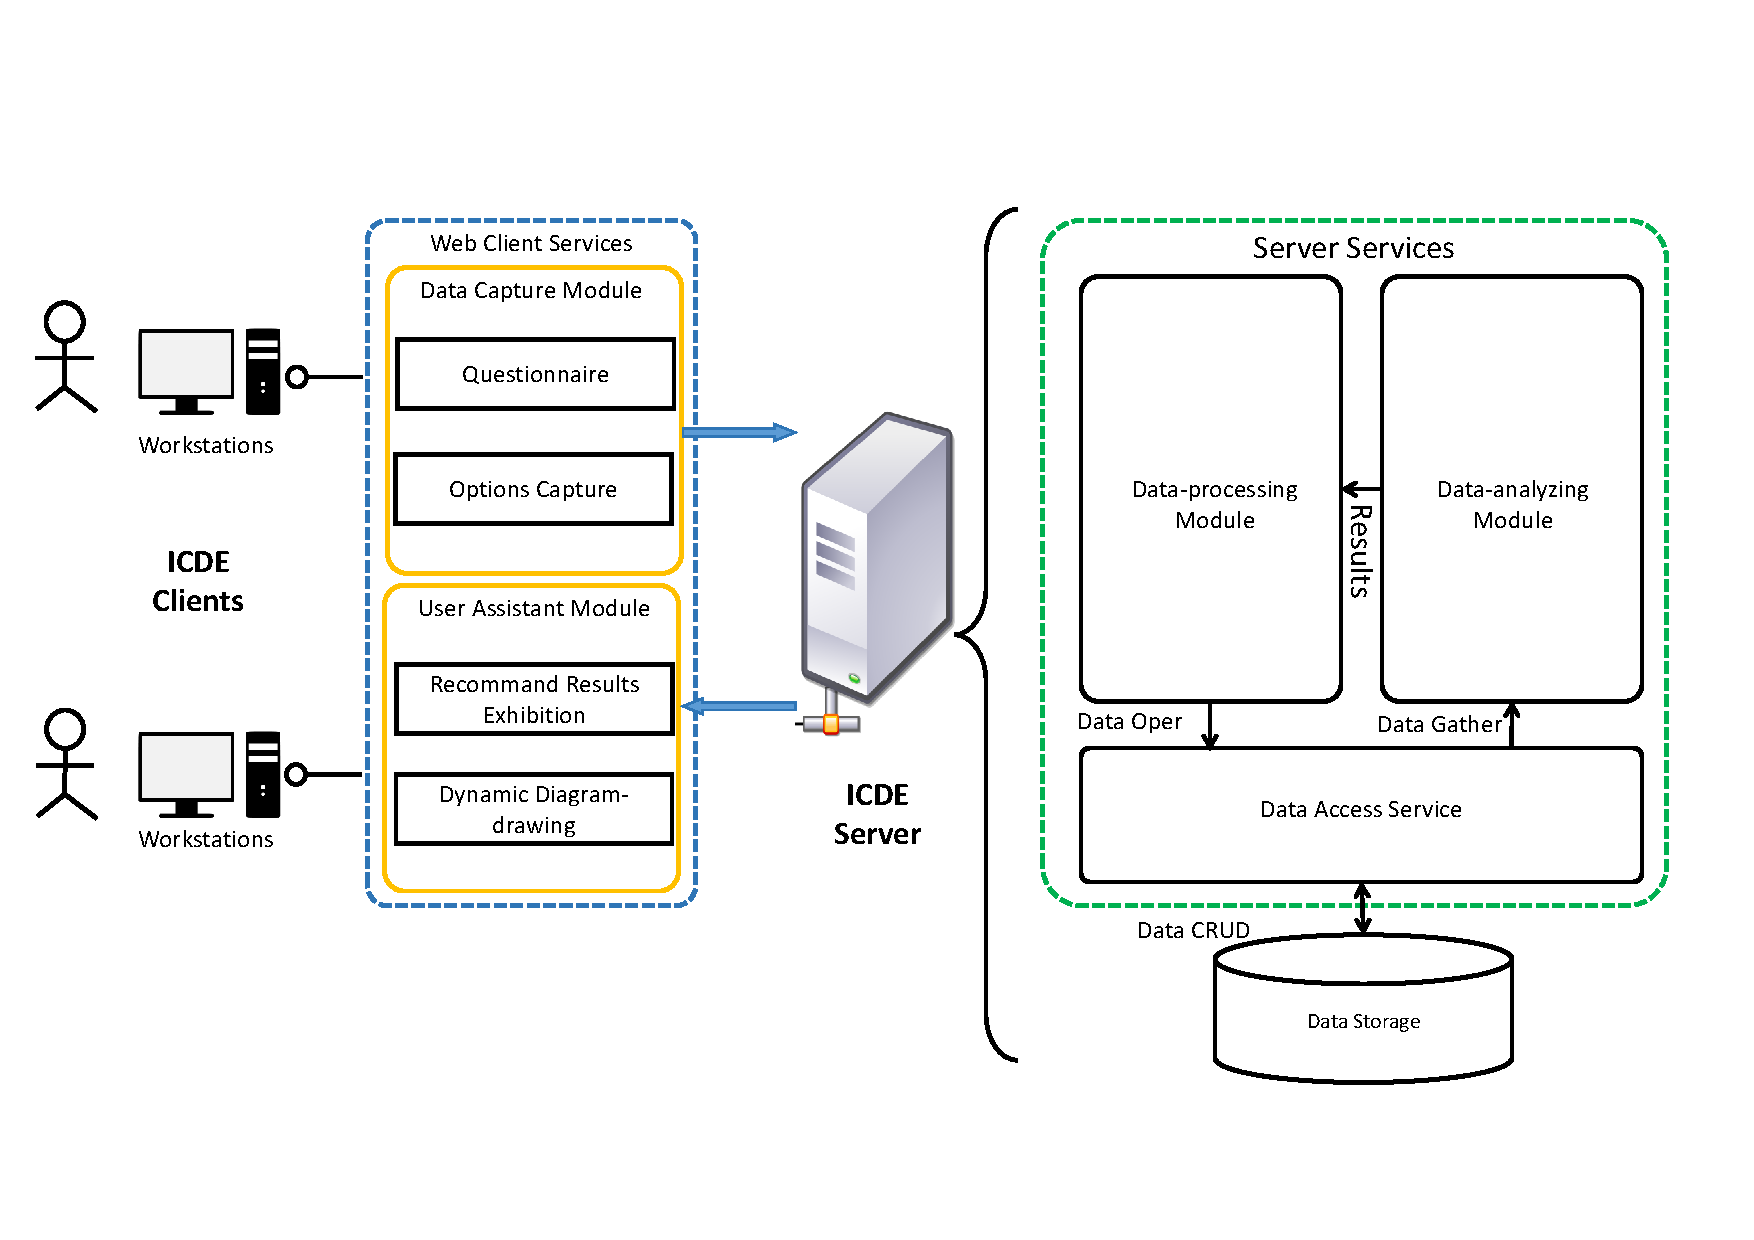
\includegraphics[width=0.9\textwidth]{Architecture.pdf}}
\caption{The high-level architecture graph of Tripedia.}
\label{high_level_arch}
\end{figure*}

\begin{figure*}[htbp]
\centerline{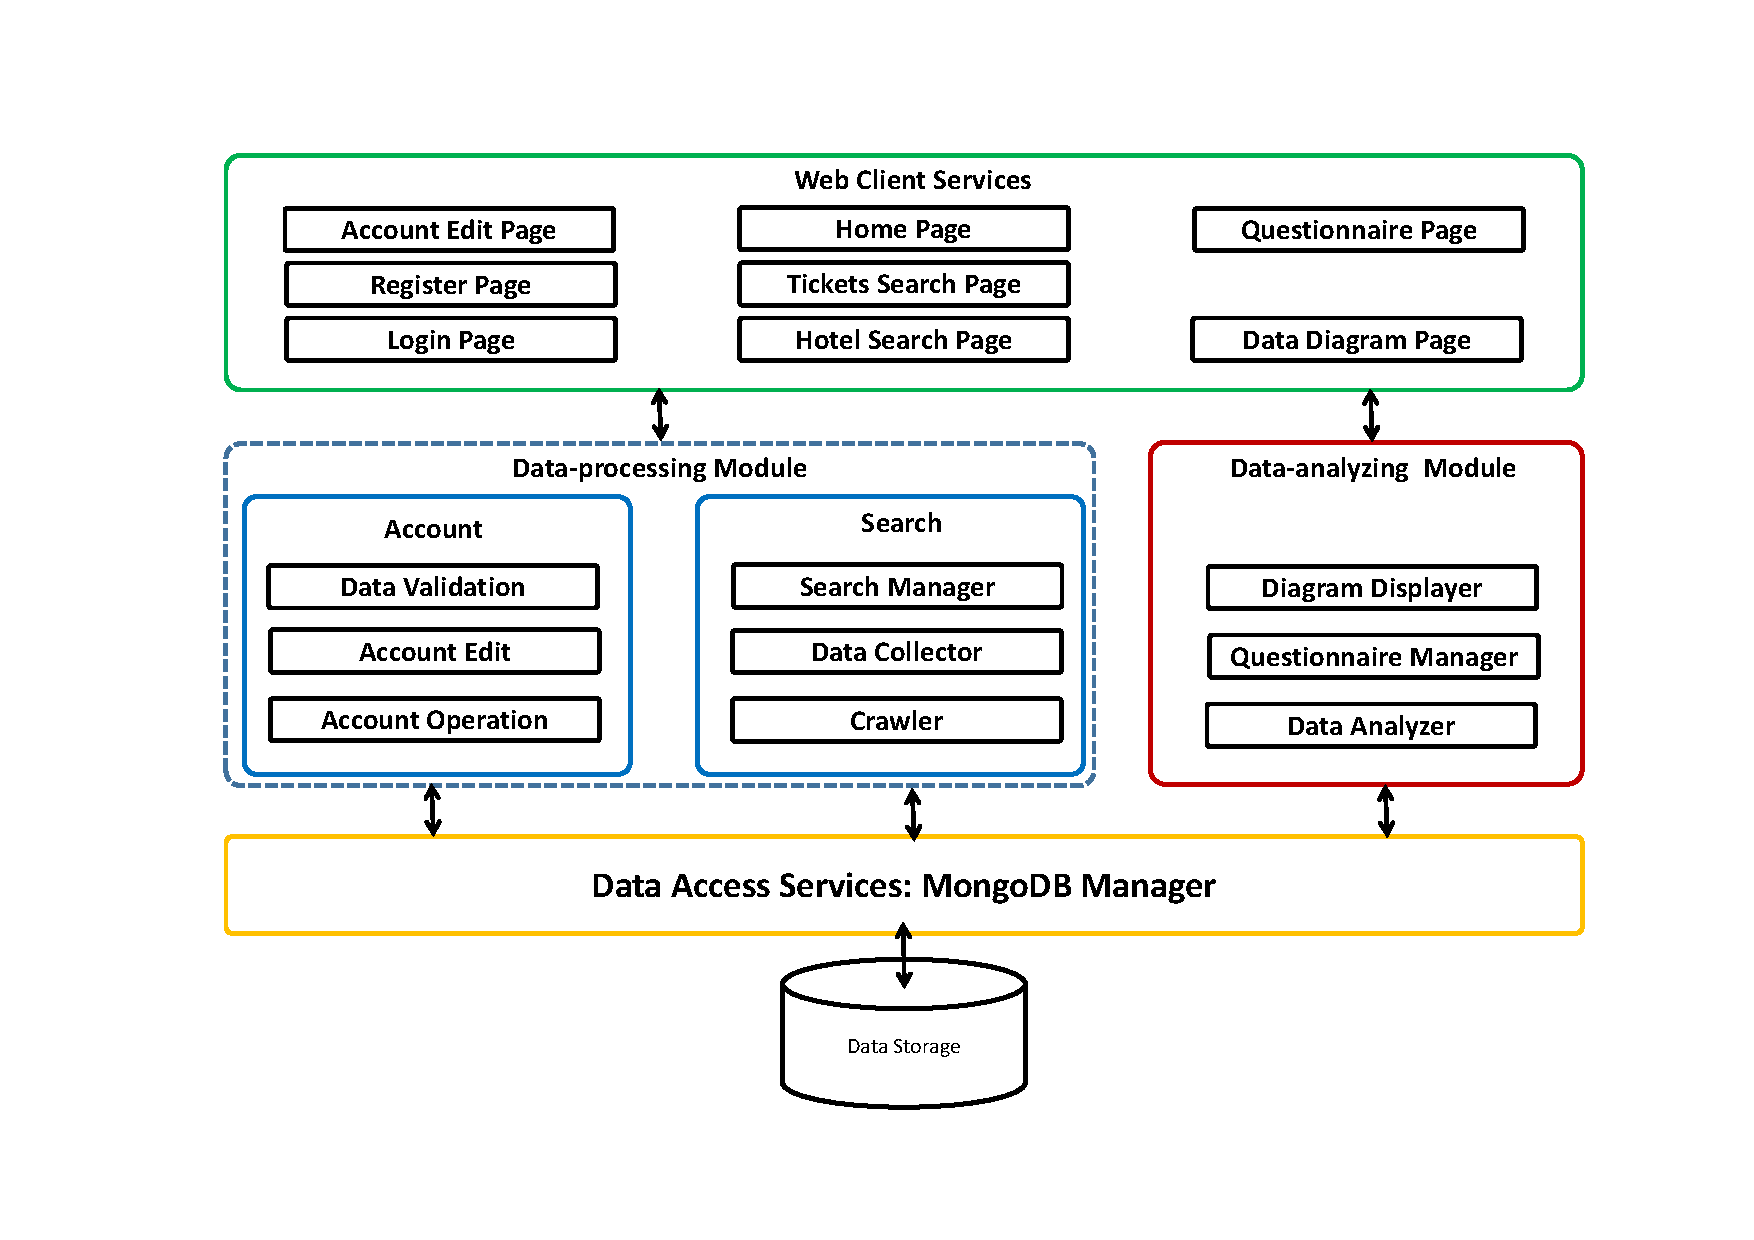
\includegraphics[width=1.0\textwidth]{Architecture2.pdf}}
\caption{The system-level architecture graph of Tripedia.}
\label{system_level_arch}
\end{figure*}




\section{\textbf{The Agile Process}}


\subsection{\textbf{Team Setup}}



\subsection{\textbf{Association between User Stories and Sub-requirements}}

\subsection{\textbf{The Scrum Sprint Cycle}}

\subsubsection{\textbf{Review Work to be done}}


\subsubsection{\textbf{Product Backlog}}

\subsubsection{\textbf{Sprint Plan}}



\subsubsection{\textbf{Sprint Backlog}}

\subsubsection{\textbf{Sprint Process}}

\subsubsection{\textbf{Sprint Review}}


\section{\textbf{Architecture}}


\subsection{\textbf{Architecture Design in Overall Level}}

As shown in Figure\ref{high_level_arch}, the high-level ICDE system architecture mainly contains two parts: client and server. Based on the limited server hardware equipment, we implement the data analysis logic as a single module in the server, which stands for ICDE 3rd Party Applications. 

In the client part, we implement Tripedia's client logic based on the web. The web client service mainly contains user assistance services and data capture services. The web pages provided by the web services are the operation interface for users.

On the server side, we will develop three modules to implement the backbone of the ICDE system: Data-processing Module, Data-analyzing Module, and Data Access Service. The Data Access Service, as the median layer for database access, provides a unified database interface (deletion, modification, query, etc) for the Data-processing Module and the Data-analyzing module. The Data-processing Module is responsible for the basic logic of the server, such as registration, login, search, data preprocessing, and other interaction logic with the client. The Data-analyzing Module accesses the data in the database through the Data Access Service to perform data analysis and returns the analysis results to the Data-processing Module.

To sum up, Tripedia's architecture is a standard ICDE system. The Client part includes a Data Capture Service to collect user behavior and information and transmit relevant data to the server. The Data-processing Module in the Servers section is responsible for implementing the interactive logic of the server; the Data Access Service provides a unified data access interface; the Data-analyzing Module serves as the core of the ICDE system to analyze user data and feedback the analysis results to the user through the server to provide User Assistance Service.


\subsection{\textbf{Architecture Design in User Requirements Level}}

The system-level architecture is shown in Figure \ref{system_level_arch}. The main layout of the system-level architecture diagram is similar to the overall level architecture diagram. The system-level architecture shows the functions in each Module in detail. Considering the features of our system, we design our system-level architecture based on Layer Information System Architecture and Processing Application Architecture.

The web client services contain a series of web pages, which provide operation interfaces for users.

The data-processing module can be divided into two parts: Account and Search. The Account part focuses on the requirements of account operation. Meanwhile, the Search part is responsible for searching data from both networks and the database.

The data-analyzing module is responsible for data analysis and diagram displaying, which play the role of data processing in the ICDE system.

The MongoDB Manager is a database operation mediate layer, which increases the reusability of the database interface.

\section{\textbf{Modeling and Design}}

In this section, we will discuss the design of the tasks of the Tripedia. For a clearer structural presentation, we consider the choice of task description granularity. A small task granularity can not take on the task of showing interactions among multiple objects. A large task granularity may lose the meaning of the task design. Therefore, we merged some sub-requirements into a single task. We try to show the relationships among objects as much as possible while ensuring appropriate granularity. 

\subsection{\textbf{Task: Login \& Register }}

\subsubsection{\textbf{Task Context }}
\textbf{}

This class diagram meticulously outlines the architecture of a user login and registration system, representing a coalescence of strategically organized classes - the 'user,' 'UserDAO,' and 'Database(MongoDB)' - each playing a pivotal role in safeguarding and proficiently managing user information.

The 'user' class is the cornerstone, embodying essential attributes such as username, password, and email alongside crucial functionalities that facilitate user login and registration processes. It acts as the primary interface, allowing users to interact with the system ensuring their credentials are accurately captured and securely managed.

The 'UserDAO' class emerges as a vital intermediary, bridging the 'user' class and the 'Database(MongoDB)' class. It encapsulates many user-related database operations, including user creation and data retrieval, fostering a seamless and efficient management of user data stored within the database.

Lastly, the 'Database(MongoDB)' class is dedicated to direct interactions with the MongoDB database, ingrained with essential attributes and functionalities required for initiating and managing connections, emphasizing the robustness and reliability of the database operations.

Together, these classes form a cohesive system aimed at simplifying the user login and registration process while prioritizing the integrity and security of user data. Through precise role allocations and harmonious class collaboration, the system is empowered to process user requests proficiently, ensuring a streamlined and secure user login and registration experience.

\subsubsection{\textbf{Structural Context }}
\textbf{}

According to the login and registration activity diagram, we elucidate the structural context and task data flow, mapping the journey of a user through the system and delineating the roles and interactions that various elements undertake during user authentication processes.

Initially, the user encounters a decision node, questioning the existence of an account. Lacking an account directs the user towards the registration process, where they populate necessary fields with relevant information, initiating a verification process and ensuring the uniqueness of the username within the system database. Once validated, the user’s data is secured in the database, concluding the registration.
If the user possesses an account, they navigate towards the login page. Here, the user enters essential login credentials - username and password. The system then validates these credentials, checking their conformity with the stored data. Incorrect details will circulate the user back to re-enter the correct credentials, while a successful validation will grant the user access, redirecting them to the homepage.

Throughout this process, each object and decision node plays a critical role in managing the data flow and ensuring secure and correct user authentication. The precise coordination and interaction among these objects and decision nodes are pivotal for a seamless and secure user experience accessing the system. The process guarantees that only registered and validated users gain access, preserving the integrity and security of the system and its data.

\subsubsection{\textbf{Interaction Context}}
\textbf{}

\textbf{Registration Process}:

The actor (user) begins registering by entering their information on the registration page.

The Register Page, upon receiving the user's information, communicates with the Server to check whether the username already exists in the Database.

The Server accesses the Database to validate the uniqueness of the username. It returns a Boolean value, indicating the existence or non-existence of the username.
If the username is available, the Server saves the user's information into the Database. A confirmation message is returned to the Register Page, informing the user of the successful registration, and the user is redirected to the login page.

\textbf{Login Process}:

For the login process, the actor enters their username and password on the Login Page.

The Login Page then passes the entered credentials to the Server for validation.
The Server cross-references the provided username and password with the stored information in the Database. The Database returns a result, confirming or denying the match of the credentials.

Depending on the result, the Server informs the Login Page of the success or failure of the login attempt, and the corresponding message is displayed to the user. In case of successful login, the user gains access to their account.

This context describes a two-part interaction where the user first registers by entering personal details, and the system validates the information. After successful registration, the user logs in with their credentials, which are verified by the system for authentication.

\subsubsection{\textbf{Behavior Context}}
\textbf{}

The state diagrams vividly encapsulate the user journey during the registration and login processes. Let us delve into the behavior context of these tasks:

\textbf{Registration}:

Enter Register Page: The journey begins with the user entering the registration page, marking the inception of the registration process.

Fill in the Information: Users are required to fill in their necessary information, such as usernames and passwords.

Verify the Username Existence: The system then verifies whether the username already exists in the database.

Username Available: If the username does not exist in the system, it proceeds to register the user successfully.

Username Existed: If the username is already taken, the registration process halts, indicating the unavailability of the chosen username.

\textbf{Login}:

Enter Username and Password: Users start by entering their username and password, initiating the login process.

Send to Server: The entered credentials are then sent to the server for verification.

Match the Data: The server matches the entered credentials against the stored data in the database.

Verify Successfully: If the credentials match, the user is verified successfully, marking a successful login.

Verify Failure: If there is a mismatch in the credentials, the verification fails, and the login process is interrupted.

In both diagrams, the transition of states is clear and systematically laid out, guiding users through each phase of registration and login, ensuring clarity and precision in navigating the website’s authentication processes.


\subsection{\textbf{Task: Account Edit }}

\subsubsection{\textbf{Task Conext }}
\textbf{ }

The class diagram in the provided figure illustrates the relationships and interactions among various entities in a user profile management system, specifically focusing on the functionalities of editing personal information and changing passwords.

Central to the diagram is the ‘User’ class, containing essential personal attributes such as username, name, password, and contact details. This class is fundamental and acts as a data structure where individual user information is stored and manipulated. The ‘User’ class has operations like ‘editPersonalInfo()’ and ‘changePassword()’ to allow users to update their information and credentials.
Collaborating closely with the ‘User’ class is the ‘Profile Manager’. The ‘Profile Manager’ acts as an intermediary facilitating various user operations. It holds a reference to the current ‘User’ and encompasses methods such as ‘loadUserInfo(),’ ‘saveUserInfo(),’ and ‘validatePassword().’ These methods are crucial for retrieving, updating, and validating user information against the database.

The ‘MongoDB connector’ class is instrumental in interfacing with the database. It encapsulates basic database operations such as connect, find, insert, update, and delete, ensuring the application can interact seamlessly with the MongoDB database.
This design promotes modularity and separation of concerns. The ‘User’ class focuses on user data, the ‘Profile Manager’ manages user interactions, and the ‘MongoDB connector’ deals with database communications. By having a dedicated class for MongoDB operations, the design ensures that changes in database technologies or schemas have minimal impact on the user management functionalities, thus enhancing maintainability and flexibility. It facilitates the easy adaptation of the system to meet evolving requirements or technologies, promoting robustness and reusability of the system components in managing user profiles effectively.

\subsubsection{\textbf{Structural Conext }}
\textbf{ }

In the discussion here, we delve into the data flow processing depicted in the modified activity diagram for user account modification, encompassing both the changing of personal information and passwords.

The user initiates the process by opting to modify the account. They are presented with two paths: one for password modification and another for editing personal information, each comprising a series of systematic steps facilitated by the system's user account management functionalities.

Password Modification Pathway:
The user navigates to the 'Change password page,' where they are prompted to enter their username and answer a secret question as a security measure.
The system validates the information entered. If it doesn't match the existing records, the user is prompted to re-enter the correct details.
Upon successful validation, the user is allowed to enter a new password, which then gets saved as part of the user's account information.
Personal Information Modification Pathway:
Users who wish to modify their personal information are directed to the 'Edit Info page.'

Here, users can input new information, like updating addresses or contact details, which the system captures and saves, ensuring the user's account information remains current and accurate.

In this structured context, each component (Modify Account, Change Password Page, and Edit Info Page) plays a pivotal role in orchestrating the flow of information, ensuring that user preferences are accurately captured, validated, and updated as per the user's inputs. The cohesive interaction between these components ensures a secure and user-friendly environment for account modification tasks, safeguarding user data while allowing flexibility for necessary updates and modifications.


\subsubsection{\textbf{Interaction Conext }}
\textbf{ }

\textbf{ Password Modification Process}:

User Interaction: The actor (user) initiates the password modification by entering their username and new password and answering a secret question on a specific webpage.

Verification and Validation: The webpage, upon capturing the user's details, interacts with the profile manager to verify the user's identity by matching the username and secret question with the records in the MongoDB database.

Password Updating: If the verification is successful, the profile manager facilitates the updating of the password in the MongoDB database. A confirmation of this update, whether successful or failed, is communicated back to the user through the webpage.

\textbf{ User Information Editing Process}:

Information Entry: The actor engages in editing their user information by inputting the necessary details on a specific webpage.

Information Transmission: The webpage takes responsibility for forwarding the modified or newly entered information to the profile manager to commence the editing process.

Database Interaction: The profile manager cooperates with MongoDB to secure the updated information, receiving a confirmation about whether the information was successfully saved or not.

Completion Confirmation: The result of the information editing process, either a success or failure, is communicated back to the actor through the webpage, concluding the interaction for editing user information.

This comprehensive interaction context illustrates a dual-functional process. It involves a password modification procedure followed by a user information editing activity, each with unique steps and interactions among various components like the user, webpage, profile manager, and MongoDB database.

\subsubsection{\textbf{Behavior Conext }}
\textbf{ }

\textbf{ Password Modification}

Initialization: The process begins when the user intends to modify the password, initializing the system to receive the necessary information.

Enter Username and Secret Question: The user provides their username and answer to a secret question to confirm identity.

Verification: The system then verifies the information. If the information is correct, the process proceeds; otherwise, the user is prompted to re-enter the details.

Password Entry and Saving: Upon successful verification, the user can enter a new password. The system will then save this new password, completing the process.

\textbf{ User Profile Editing}

Initialization: The process commences with the system ready to receive updated user information.

Enter UserInfo: Users enter or edit their personal information in the provided fields.

Information Transmission: The edited information is sent to the server for processing and validation.

Database Interaction: After successful validation, the information is saved in the database, and a confirmation is generated.

Completion: Finally, a success message is displayed to the user, indicating that the edits have been successfully made and saved.

Each state transition is systematic and user-friendly, ensuring that the users find the process intuitive and straightforward. Both processes are designed to secure user data and ensure that changes are made correctly and effectively.



\subsection{\textbf{Task: Searching Data from Database }}


\subsubsection{\textbf{Task Conext }}

\textbf{}

The class diagram in Figure \ref{class1} shows the relationships among the searcher and database manager. 

The DBManager is a base class in the database interface, which encapsulates the Mongo Database interface. The DBManager can search hotel data and ticket data from the database.

The Searcher class is responsible for catching the keywords that users want to search for. Then call DBManager to find the data in the database based on the keywords combined into a query statement.

Above all, we have designed the context of the diagram display task.
\begin{figure}[htbp]
	\centerline{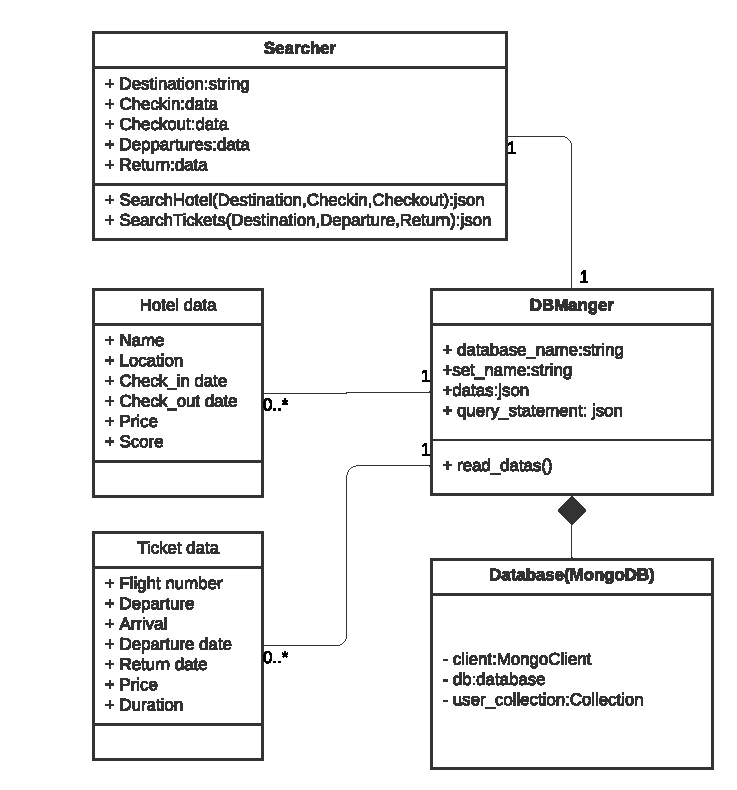
\includegraphics[width=0.5\textwidth]{image/searching hotel class1.pdf}}
	\caption{Class diagram of Searching data from database }
	\label{class1}
\end{figure}

\subsubsection{\textbf{Structural Conext }}

\textbf{}

In this section, we discuss the data flow processing by Figure \ref{activity1}. Meanwhile, we show the roles these objects play in the data flow processing, which describes the structural context of the Searching Data from Database task.

The user enters the keyword on the search page. Then the service combines the keyword into a query statement. DBManager searches the data from the database based on the query statement. Finally, the Searcher shows the data in the front end.
\begin{figure}[htbp]
	\centerline{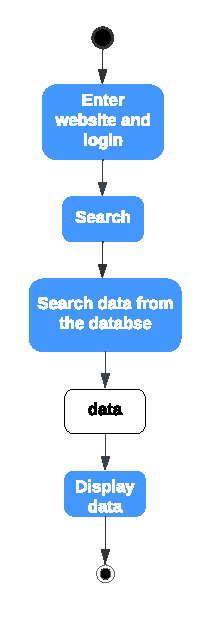
\includegraphics[width=0.5\textwidth]{image/searching hotel activity1.pdf}}
	\caption{Activity diagram of Searching data from database }
	\label{activity1}
\end{figure}


\subsubsection{\textbf{Interaction Conext }}
\textbf{}

The sequence diagram in Figure \ref{sequence1} shows the interaction context of this task. 

The user inputs the keyword and calls the SearchHotel function or Search Ticket function of the Searcher object. The Searcher object calls the read\_data function provided by the DBManager object to get the related data from the database.

In the end, the Searcher Object displays the data to the user.
\begin{figure}[htbp]
	\centerline{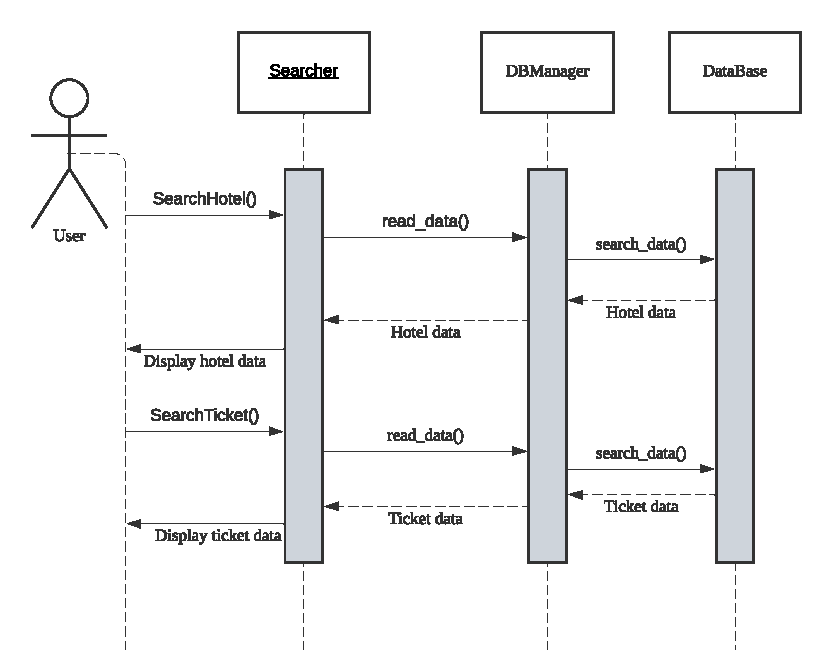
\includegraphics[width=0.5\textwidth]{image/searching hotel sequence1.pdf}}
	\caption{Sequence diagram of Searching data from database }
	\label{sequence1}
\end{figure}

\subsubsection{\textbf{Behavior Conext }}

\textbf{}

The state diagram in figure \ref{statement1} shows the behavior context of this task. 

The user enters the search web page.  After inputting the keywords, the system searches data from the database. Subsequently, the website displays the data as a list. 

\begin{figure}[htbp]
	\centerline{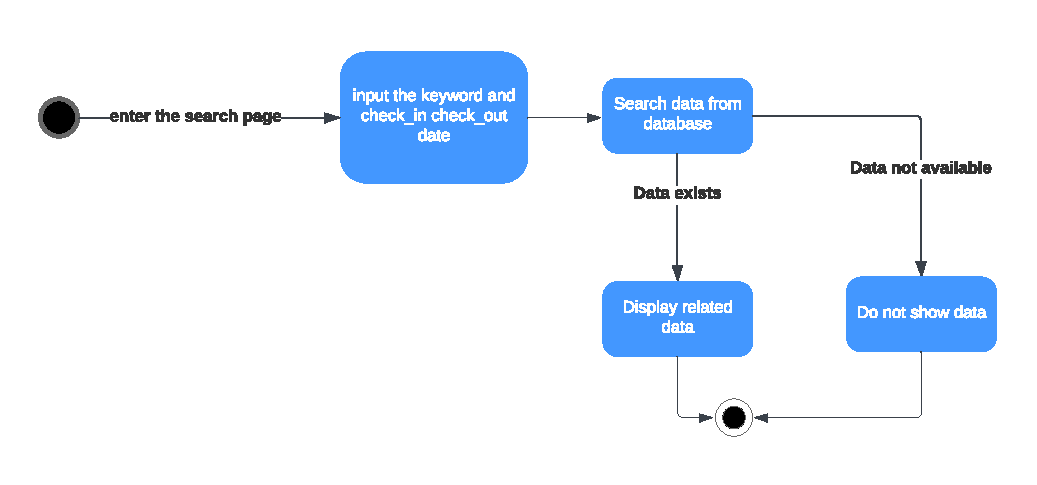
\includegraphics[width=0.5\textwidth]{image/searching hotel statement1.pdf}}
	\caption{Statement diagram of Searching data from database }
	\label{statement1}
\end{figure}

\subsection{\textbf{Task: Crawler searching }}



\subsubsection{\textbf{Task Conext }}
\textbf{}

The class diagram in Figure \ref{crawlerclass1} shows the relationships among the searcher, crawler and database manager. 

The DBManager is a base class in the database interface, which encapsulates the Mongo Database interface. The DBManager can save hotel data and ticket data into the database.

The Searcher class is responsible for catching the keywords that users want to search for. When the searcher receives the keywords, it will call the Crawler to search information from the internet.

The Crawler class is responsible for catching data from the internet. The Crawler can be generalized as the HotelCollector and TicketsCollector. They have extended with some class functions related to searching hotel or ticket data from the internet.  When they get hotel and ticket data, they will call the DBManager to save the data into the database.
\begin{figure*}[htbp]
	\centerline{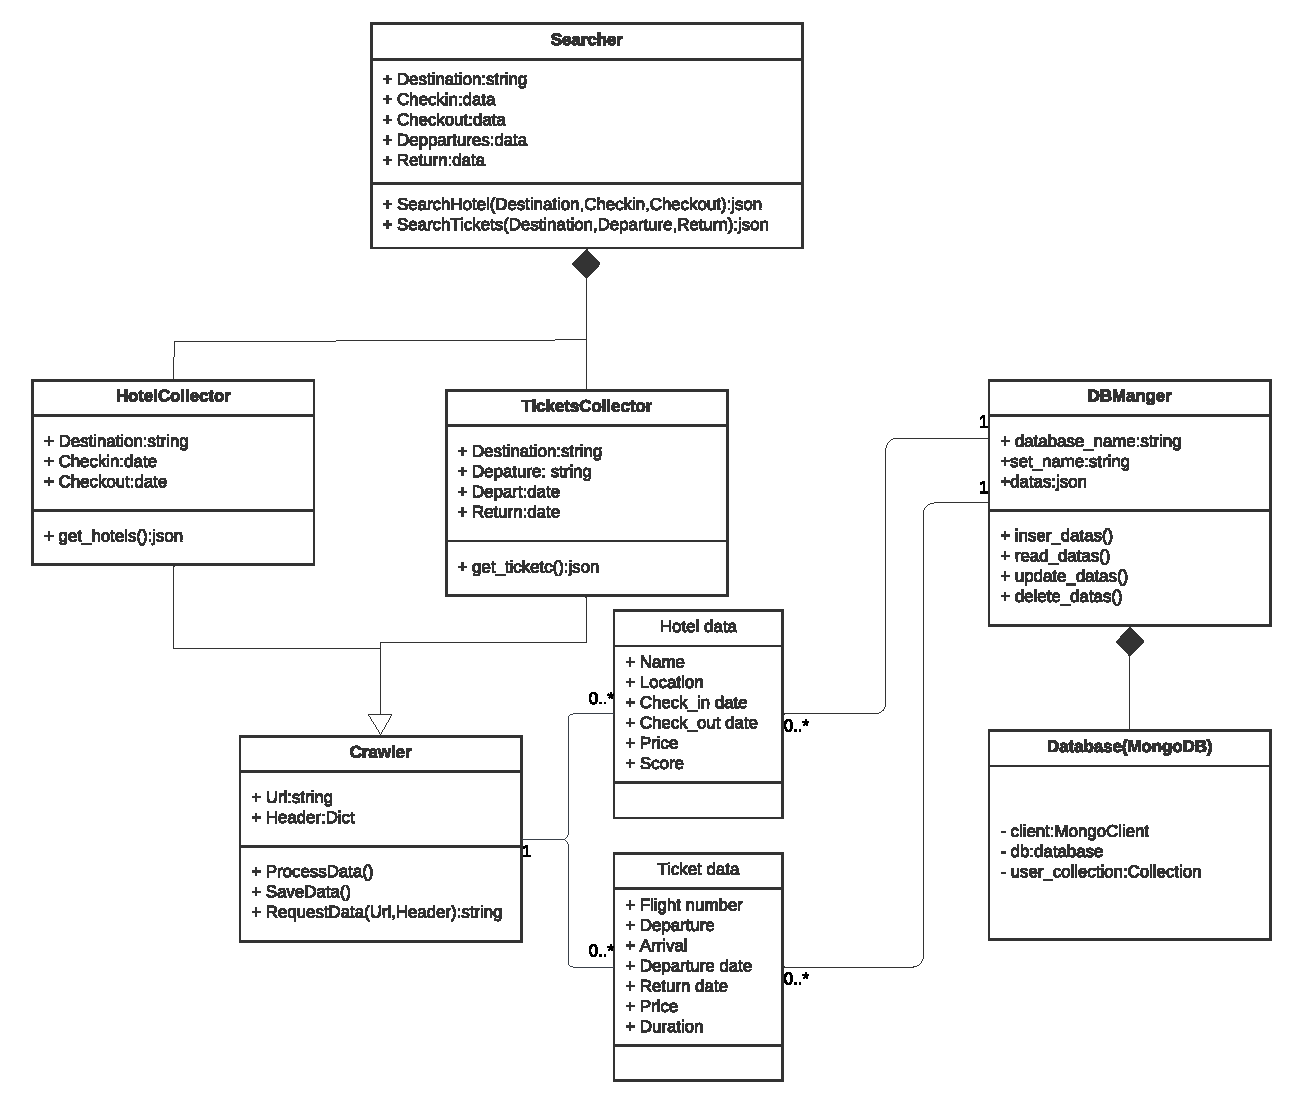
\includegraphics[width=0.9\textwidth]{image/crawler search class1.pdf}}
	\caption{Class diagram of Crawler searching }
	\label{crawlerclass1}
\end{figure*}

\subsubsection{\textbf{Structural Conext }}
\textbf{}

In this section, we discuss the data flow processing by Figure \ref{crawleractivity1}. Meanwhile, we show the roles these objects play in the data flow processing, which describes the structural context of the Crawler searching task.

The user enters the keyword on the search page. Then the service calls the Crawler to search data from the internet. Finally, the Searcher shows the data in the front end, meanwhile, the DBManager saves the data into the database.
\begin{figure}[htbp]
	\centerline{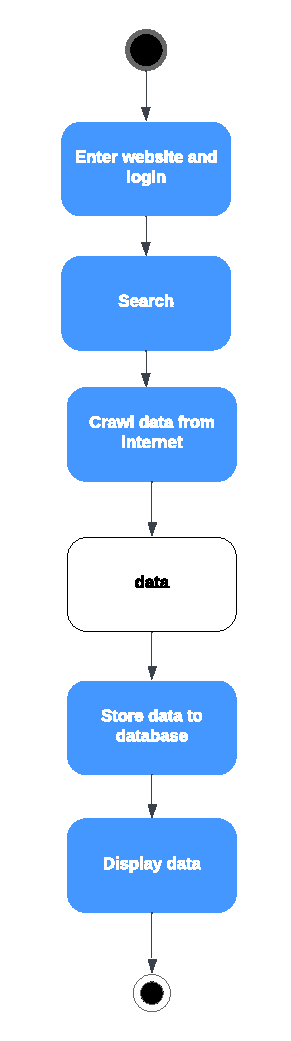
\includegraphics[width=0.5\textwidth]{image/crawler activity1.pdf}}
	\caption{Activity diagram of Crawler searching }
	\label{crawleractivity1}
\end{figure}


\subsubsection{\textbf{Interaction Conext }}
\textbf{}

The sequence diagram in Figure \ref{crawlersequence1} shows the interaction context of this task. 

The user inputs the keyword and calls the SearchHotel function or Search Ticket function of the Searcher object. The Searcher object calls the get\_hotels pr get\_tickets function provided by the Crawler object to get the related data from the Internet.

The crawler first gets the searchid from the website, and then uses the searchid to get the required data. When the Crawler receives the data, it will call the DBManager to insert it into the database and return the data to the Searcher Object.

In the end, the Searcher Object displays the data to the user.
\begin{figure}[htbp]
	\centerline{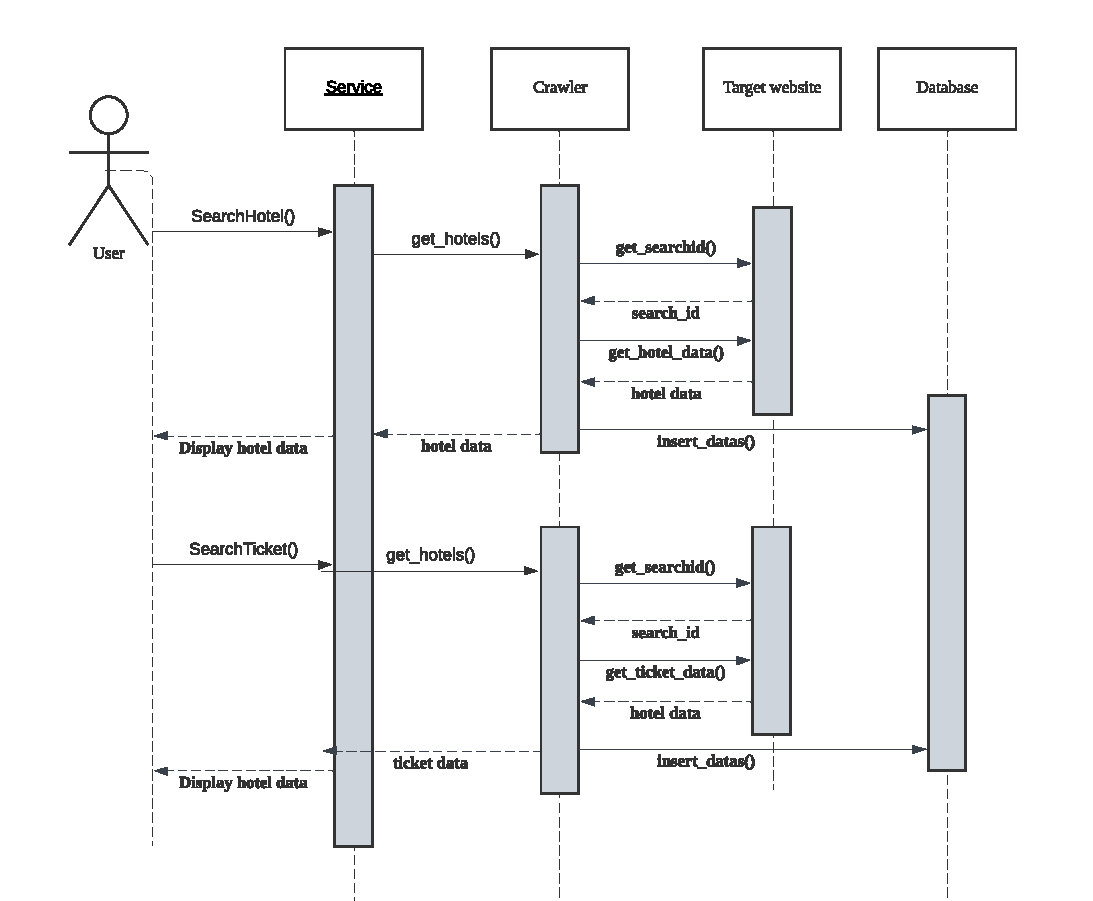
\includegraphics[width=0.5\textwidth]{image/crawler searching sequence1.pdf}}
	\caption{Sequence diagram of Crawler searching }
	\label{crawlersequence1}
\end{figure}
\subsubsection{\textbf{Behavior Conext }}
\textbf{}

The state diagram in figure \ref{crawlerstatement1} shows the behavior context of this task. 

The user enters the search web page.  After inputting the keywords, the system will call the crawler to search data from the internet. Subsequently, the website displays the data as a list and saves the data into the database.

\begin{figure}[htbp]
	\centerline{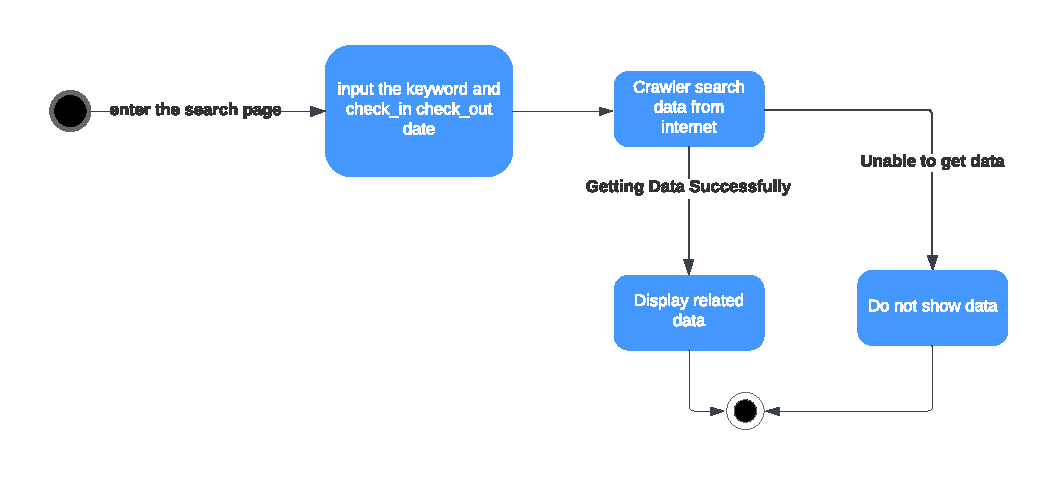
\includegraphics[width=0.5\textwidth]{image/crawler searching statement1.pdf}}
	\caption{Statement diagram of Crawler searching }
	\label{crawlerstatement1}
\end{figure}



\subsection{\textbf{Task: The Analysis Diagram}}


\subsubsection{\textbf{Task Conext }}

\textbf{}

\begin{figure*}[htbp]
\centerline{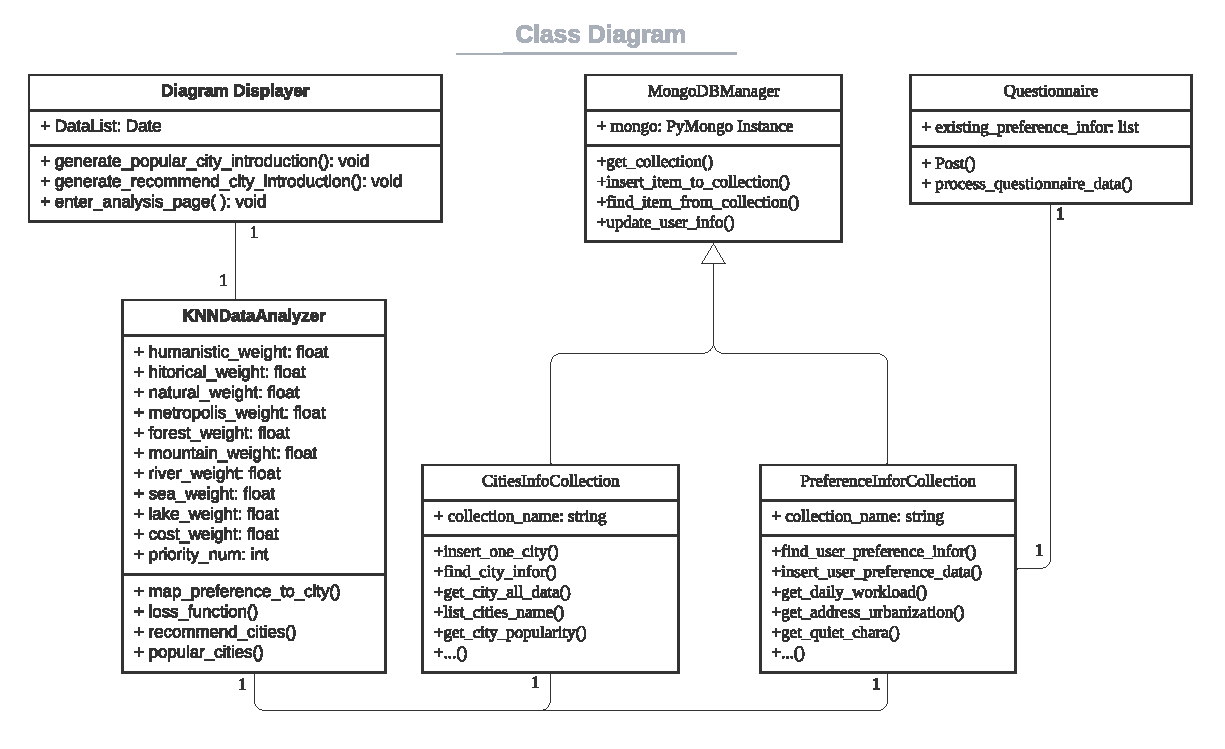
\includegraphics[width=1.0\textwidth]{diagram_structual_context.pdf}}
\caption{The class diagram of analysis diagram task.}
\label{fig_diagram_class}
\end{figure*}

The class diagram in Figure \ref{fig_diagram_class} shows the relationships among the analyzer, questionnaire, displayer, and database manager. 

For high efficiency and reusability, we designed a mediate layer for accessing the database. The MongoDBManager is a base class in the database interface, which encapsulates the Mongo Database interface. The Mongo DB Manager can be generalized as the Cities Information Collection and Preference Information Collection. The Cities Information Collection has extended with some class functions related to the city information. Meanwhile, the Preference Information Collection has extended with some class functions related to user preference information.

The Questionnaire class is responsible for catching user's preference information. A global Preference Infor Collection class instance provides the database interface for the data processing function in the Questionnaire class. Hence, the Preference Information Collection is associated with the Questionnaire.

On the other side of the class diagram, the diagram displayer performs the issues about analysis data displaying, which is based on the data analyzed by the KNNDataAnalyzer. The KNN Data Analyzer compares each city data entry with the user's preference and decides which city is the most appropriate recommendation. In this process, the KNN Data Analyzer calls the database interfaces provided by the Cities Information Collection and Preference Information Collection.

Above all, we have designed the context of the diagram display task.



\begin{figure*}[htbp]
\centerline{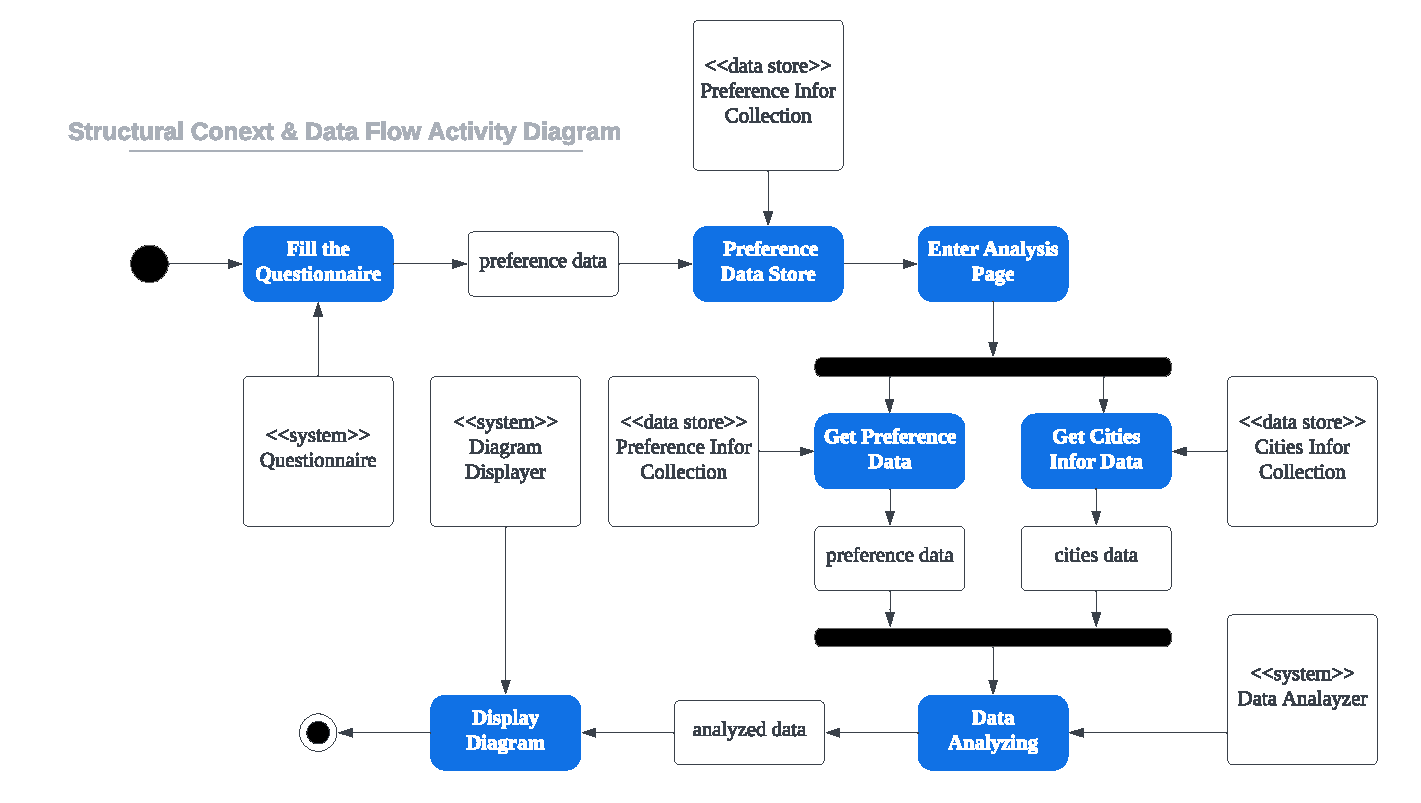
\includegraphics[width=1.0\textwidth]{diagram_data_flow.pdf}}
\caption{The structural context and data flow of analysis diagram task.}
\label{diagram_data_flow}
\end{figure*}

\subsubsection{\textbf{Structural Conext and Task Data Flow}}

\textbf{}

In this section, we discuss the data flow processing by Figure \ref{diagram_data_flow}. Meanwhile, we show the roles these objects play in the data flow processing, which describes the structural context of the Analysis Diagram task.

The user fills out the questionnaire on the questionnaire web page with the help of the questionnaire system. The Preference Information Collection saves the user's preference information for further analysis. Subsequently, the user enters the analysis page, which calls the Get Data Functions of Preference Information Collection and Cities Information Collection simultaneously. The preference data and city data are sent to the Data Analyzer for data analysis. Finally, the Diagram Displayer shows the data diagram based on analyzed data.


\begin{figure*}[htbp]
\centerline{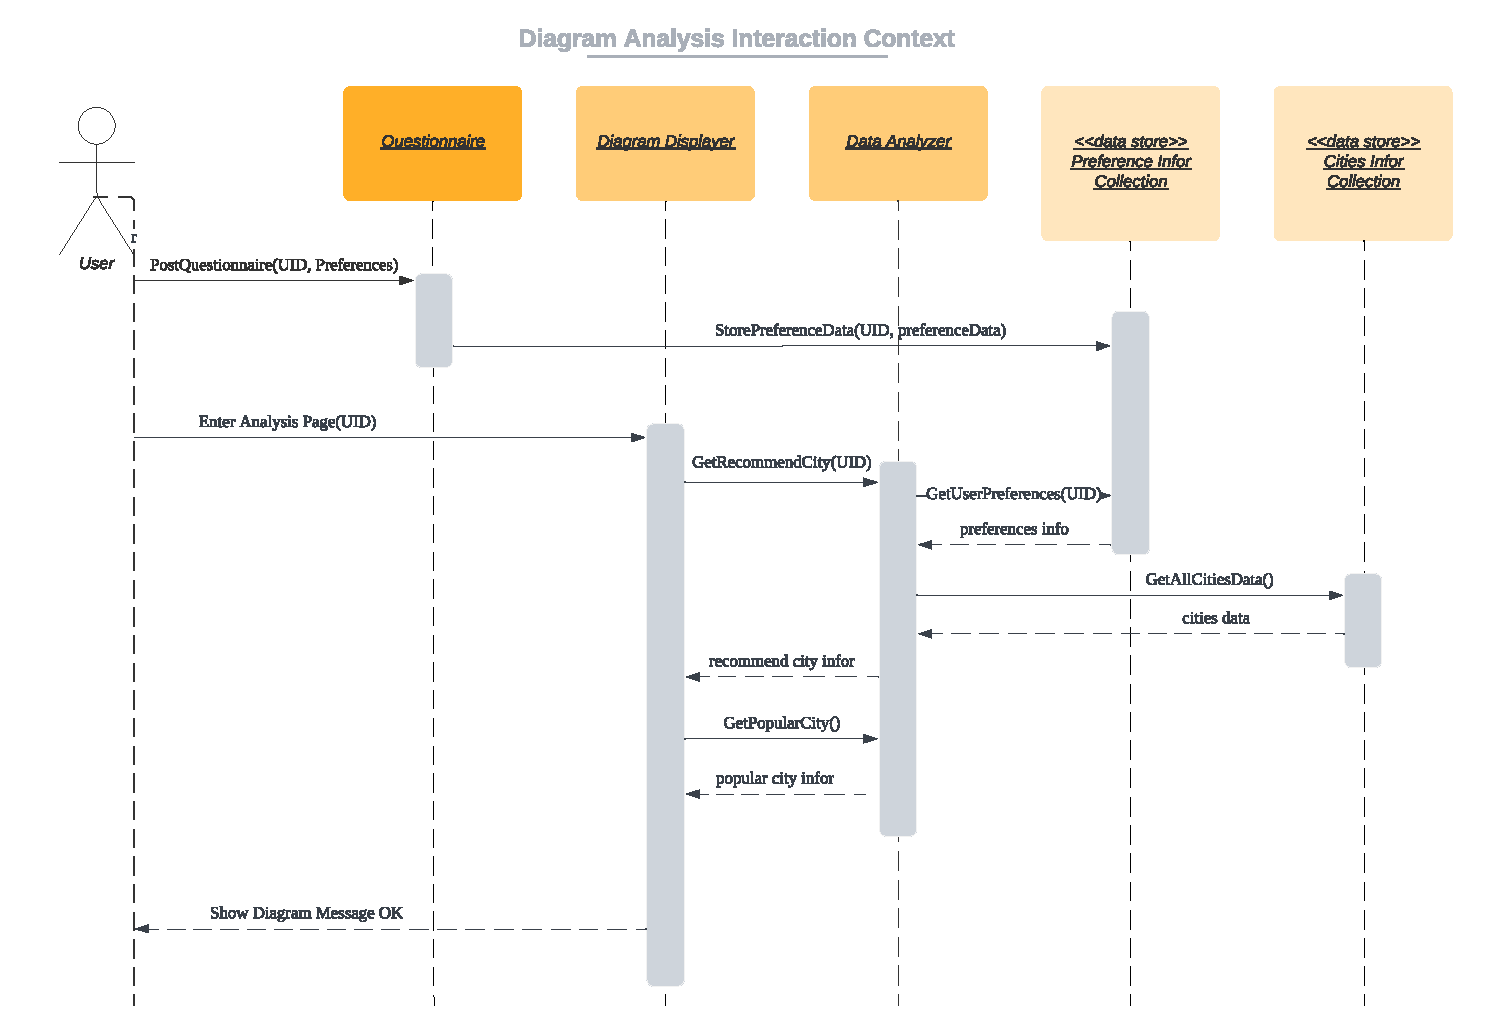
\includegraphics[width=1.0\textwidth]{diagram_interaction_context.pdf}}
\caption{The interaction context of analysis diagram task.}
\label{diagram_interaction}
\end{figure*}

\subsubsection{\textbf{Interaction Conext }}

\textbf{}

The sequence diagram in Figure \ref{diagram_interaction} shows the interaction context of this task. 

The user fills out the questionnaire and calls the PostQuestionnaire function of the Questionnaire object. The Questionnaire object calls the StorePreferenceData function provided by the Preference Infor Collection object to save the preference data into the database. 

Then the user clicks the 'recommend' button on the home page and calls the EnterAnalysisPage function, which is provided by the Diagram Displayer object. The Diagram Displayer object makes a request to the Data Analyzer for the recommendation information. The Data Analyzer gets the user preference data from the Preference Infor Collection object according to the UID. Meanwhile, all city data is gained from the Cities Infor Collection object. The Data Analyzer processes a recommendation algorithm based on these data and feeds back the recommended city information and popular city information. The Diagram Displayer shows the data diagram and returns an OK message to the user.


\begin{figure}[htbp]
\centerline{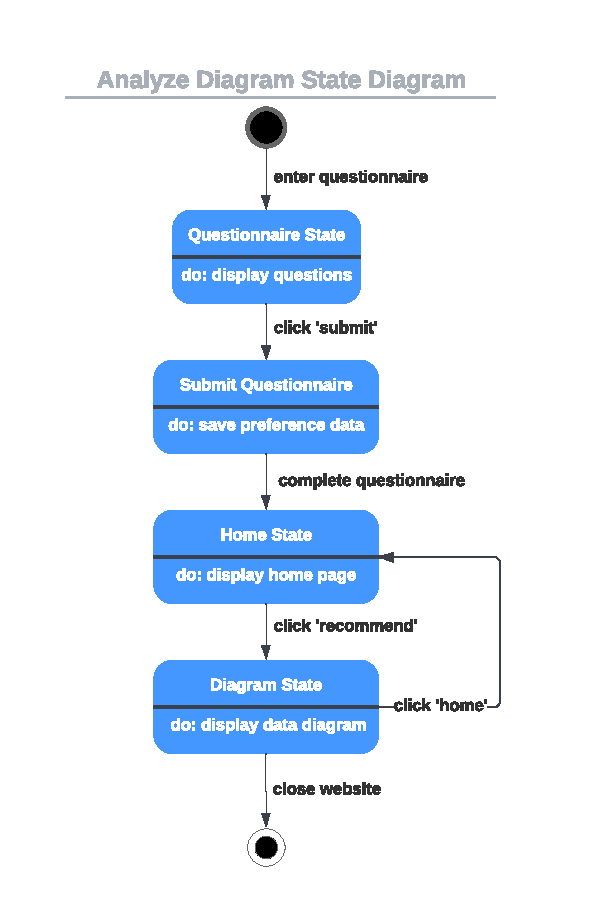
\includegraphics[width=0.5\textwidth]{diagram_state_diagram.pdf}}
\caption{The state diagram of analysis diagram task.}
\label{diagram_state_diagram}
\end{figure}


\subsubsection{\textbf{Behavior Conext }}

\textbf{}

The state diagram in figure \ref{diagram_state_diagram} shows the behavior context of this task. The state transition is simple and most functions in this task process data invisible to users. We divide the state according to the function of the web page. In this section, we only care about the states related to the analysis diagram task.

The user enters the questionnaire web page, the system enters into the Questionnaire State. The Questionnaire State displays the multiple psychological questions for users. After finishing the questionnaire, the system saves the preference data into the database. Subsequently, the website comes back to the home page and the system enters the home state. When the user clicks the 'recommend' button, the website jumps to the Analysis Diagram Page. After the system completes the recommendation, the Analysis Diagram Page displays the data diagram. 



\section{\textbf{Uncompleted Task Design }}


\subsubsection{\textbf{Task Conext }}


\subsubsection{\textbf{Structural Conext }}


\subsubsection{\textbf{Interaction Conext }}


\subsubsection{\textbf{Behavior Conext }}



\begin{figure*}[htbp]
\centerline{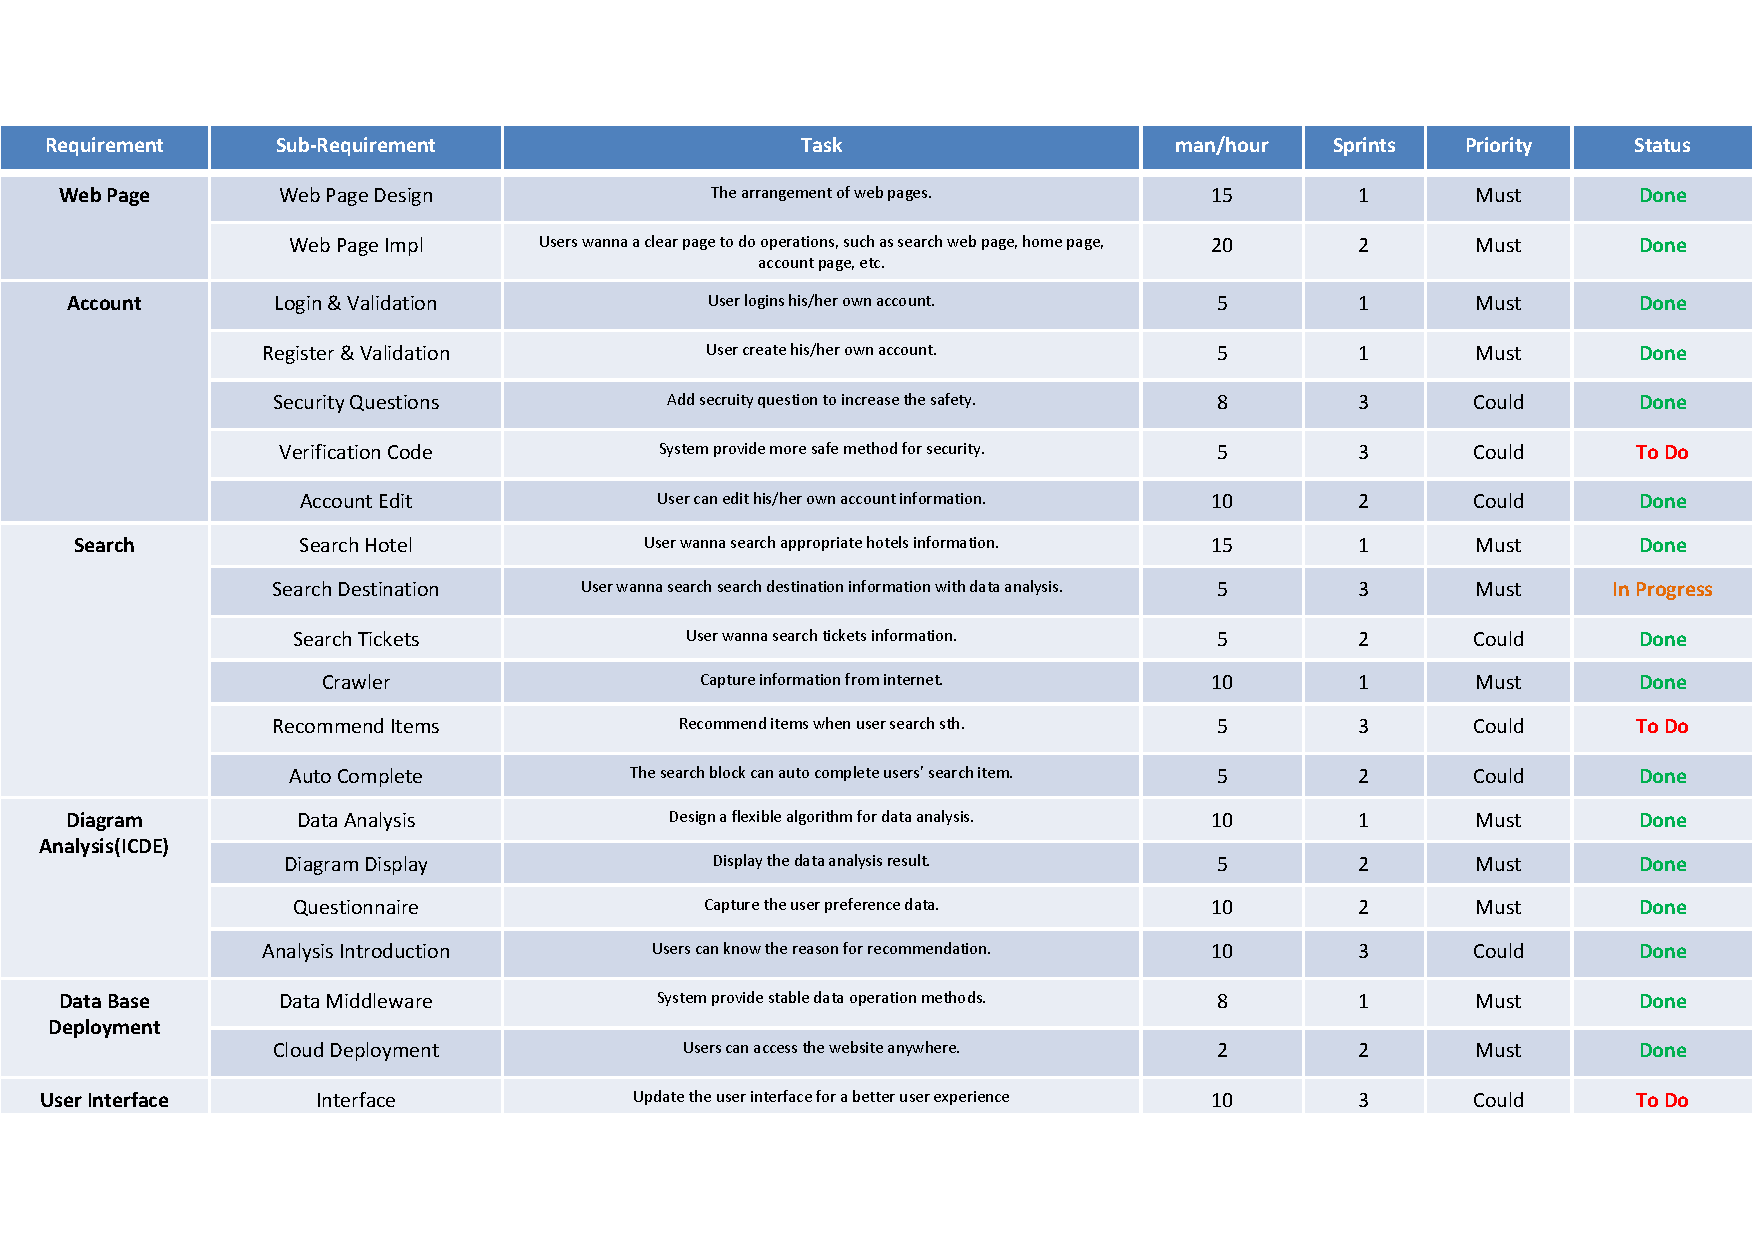
\includegraphics[width=1.0\textwidth]{dev_process.pdf}}
\caption{The development process of our system.}
\label{dev_task_diagram}
\end{figure*}


\section{\textbf{Progress Evaluation \& Analysis }}

As shown in Figure \ref{dev_task_diagram}, we have experienced two sprint cycles right now. We are designing the requirements for the next two sprint cycles(the 3rd and 4th sprint cycles).

\begin{itemize}
\item[*] The first sprint cycle: 18th September - 16th October
\item[*] The second sprint cycle: 17th October - 30th October
\item[*] The third sprint cycle: 30th October - 20th November
\end{itemize}

In the first sprint cycle, we have developed a series of basic features with MUST priority, such as Home Page, Diagram Display, Crawler, etc. In this stage, we focus on the development work of basic infrastructure, such as the crawler, and database interface encapsulation. Based on the stable architecture, we have developed an initial version system and satisfied the requirements of the ICDE.

In the second sprint, we increased the functions to boost the user experience. For example, users can edit their accounts in the second version. Meanwhile, users can search for hotels and tickets in the second system. Moreover, the data analyzer not only provides the analyzed results of the recommendation but also tells users why the recommendation is the best. At the same time, we have fixed a great number of bugs in our system.

We decided to develop the Search Destination requirement in Sprint Cycle 2. However, we face the difficulty of how to use the analyzed result to influence the search result. Hence, we modify this task to the Sprint Cycle 3. Meanwhile, we have a plan to optimize our system user interface. These works will be done in the next stage.

Above all, the development process of Goupe 7 is steady and fast. We try our best to use the software engineering technique to boost our development process, which gains a surprising result right now.










\end{document}
